\section{Parking Gate System}
\label{sec:parking_gate_system}

As already mentioned in the previous sections, the focus of this assignment is to model a parking gate system using finite state machines (FSMs).

\subsection{Requests}
\label{subsec:requests}

The requests that the parking gate system has to fulfil are the following:

\begin{itemize}
    \item Analyze the provided \textit{Vehicle FSM} and understand how it works;
    \item Define the \textit{raise} and \textit{lower} functions of the gate respecting $w_{max} = |4| [^\circ / s]$ and $\dot{w}_{max} = |1| [^\circ / s^2]$;
    \item Define the FSM to model the parking gate control system;
    \item Integrate the \textit{Vehicle FSM} and the parking gate control system FSM;
    \item Provide results of the simulation of the integrated system;
\end{itemize}

Notice that despite the suggestion from the professor to start from the already provided \textit{Vechicle FSM}, I decided to start from scratch in order to develop a deepened understanding of the FSMs, modelling also events, slightly more complex logics and composition / decomposition patterns.



\subsection{System Overview}
\label{subsec:system_overview}

The parking gate system is composed of a single Finite State Machine (FSM) that is responsible for modelling at the same time the vehicle and the parking gate system.

\begin{figure}[H]
    \centering
    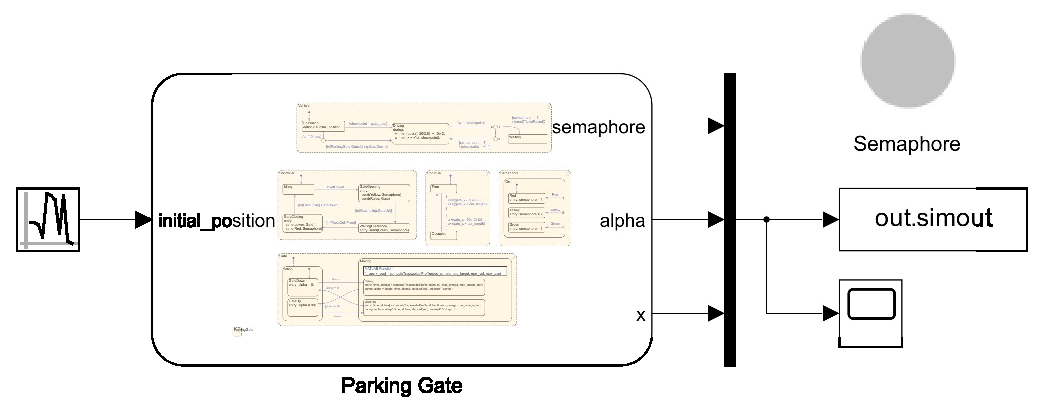
\includegraphics[width=1.0\textwidth]{./img/MATLAB/parking_gate_system_overview.pdf}
    \caption{Parking Gate System Overview}
    \label{fig:parking_gate_system}
\end{figure}

Under the hood of the unique FSM, the system is composed of other two parallel FSMs, with precise and well-defined roles and responsibilities.
The communication between the two FSMs is done through events and state transitions, which are used to inform each other about the current state of the system and to trigger the appropriate actions.

\begin{itemize}
    \item The \textit{Vehicle FSM} share the \textit{vehicle\_position (x)} with the \textit{Parking Gate FSM} to inform it about the vehicle's position in the parking lot;
    \item The \textit{Parking Gate FSM} share the \textit{semaphore\_state} with the \textit{Vehicle FSM} to inform it about the state of the gate (closed, opening, opened);
    \item The \textit{Vehicle FSM} also sends the event about the \textit{TicketPayed} to the \textit{Parking Gate FSM} to inform it that the vehicle has paid for the ticket and is ready to leave the parking lot;
\end{itemize}

Figure \ref{fig:parking_gate_system} shows the top level of the parking gate system, while Figure \ref{fig:parking_gate_system_fsm} shows the parking gate system FSM.

\begin{figure}[H]
    \centering
    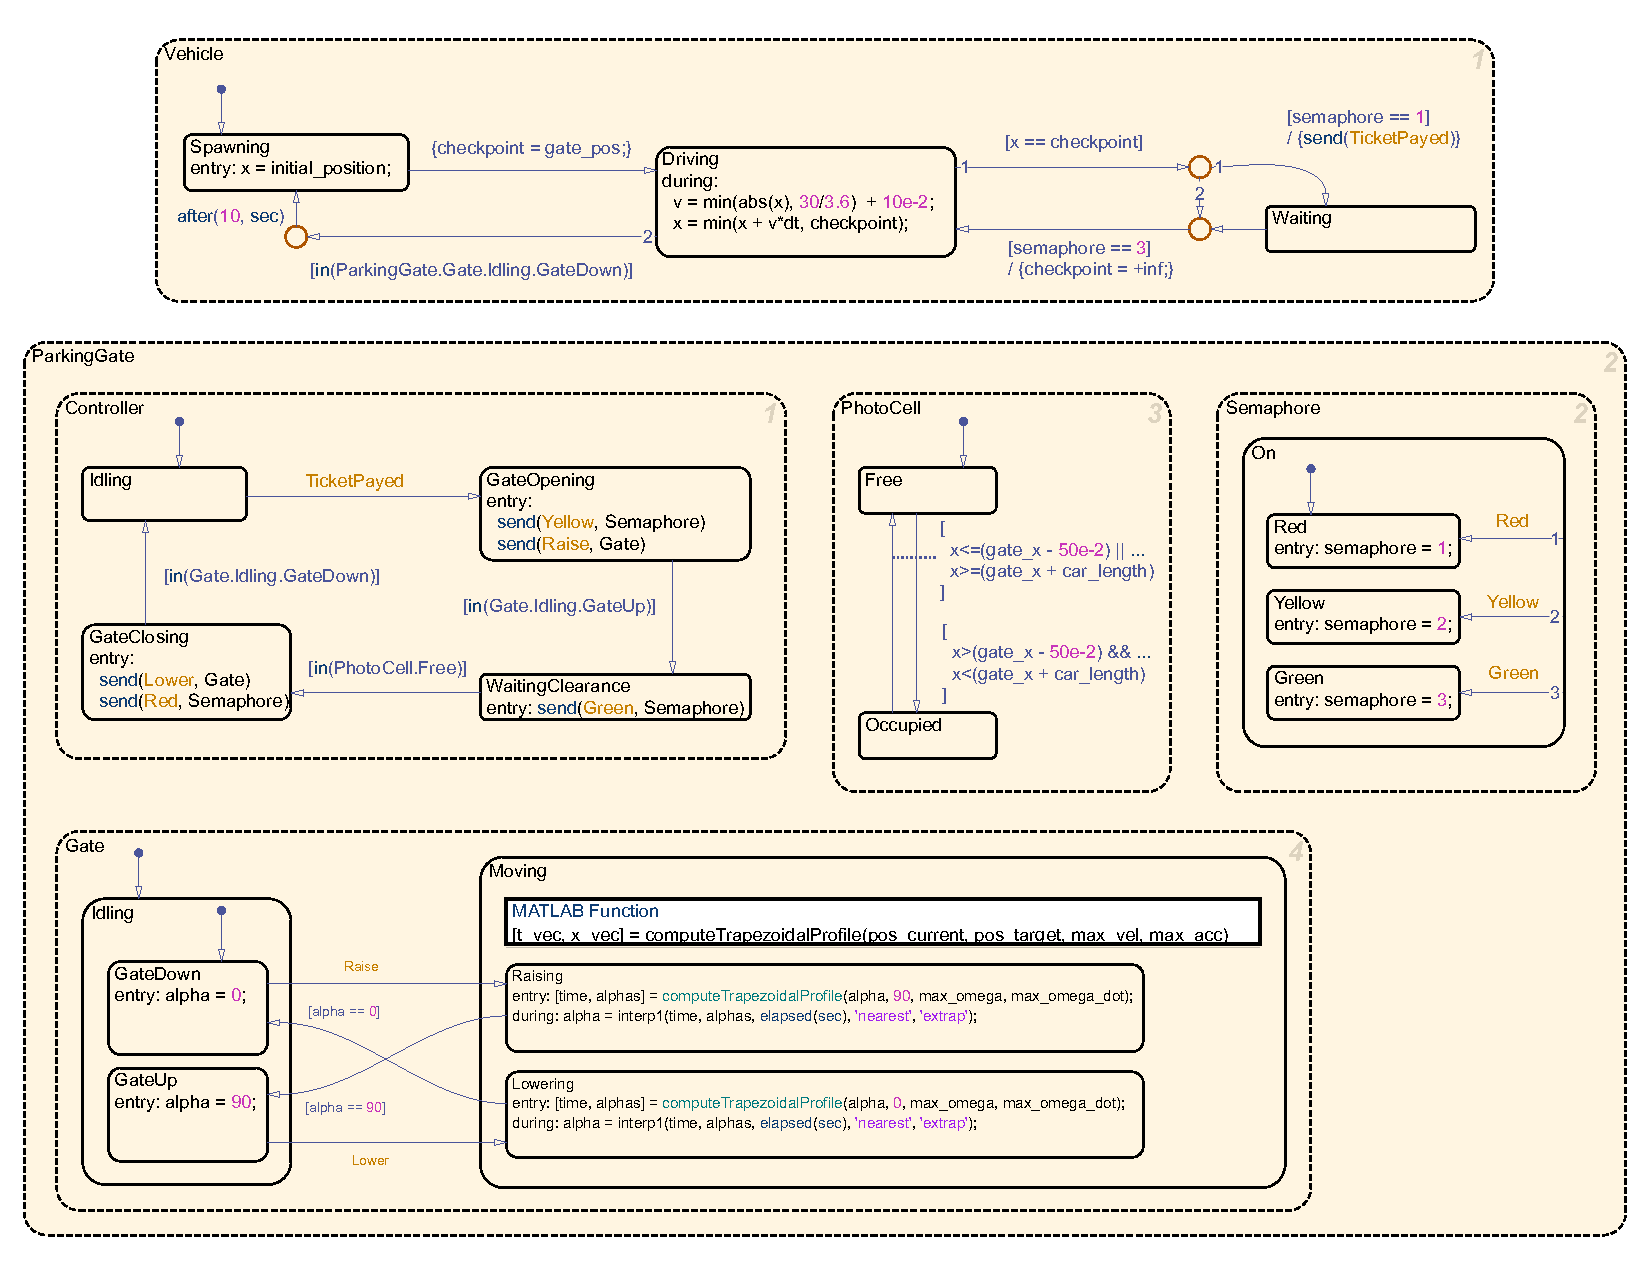
\includegraphics[width=1.0\textwidth]{./img/MATLAB/FSM_parking_gate_system_overview.pdf}
    \caption{Parking Gate System FSM}
    \label{fig:parking_gate_system_fsm}
\end{figure}



\subsubsection{Vehicle FSM}
\label{subsubsec:vehicle_fsm}

The vehicle FSM is responsible for simulating the vehicle's behavior in the parking lot.
It has two main states: \textit{Driving} and \textit{Waiting}.
At first, the vehicle is initialized and given a random position ahead of the gate.
A checkpoint is also set so that it will stop at the gate before proceeding to the next state.
Once at the gate, the vehicle looks for the semaphore state: if the semaphore is green, it directly returns to the \textit{Driving} state and proceeds ahead to the next checkpoint which is now set to $+\infty$; instead, if the semaphore is red, it simulates the payment of the ticket by sending the event \textit{TicketPayed} to the parking gate FSM and goes into the \textit{Waiting} state, waiting for the semaphore to turn green.
The vehicle proceed until the gate is closed again, when the external environment resets the vehicle to a new random position ahead of the gate to start the process again.

Figure \ref{fig:vehicle_fsm} shows the vehicle FSM.

\begin{figure}[H]
    \centering
    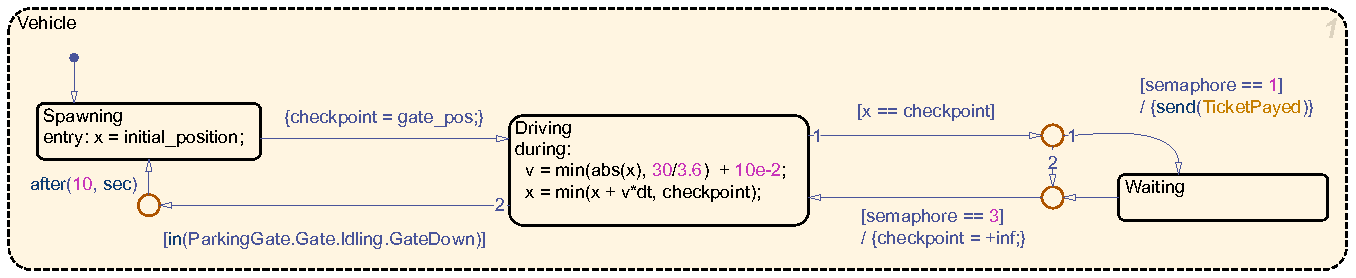
\includegraphics[width=1.0\textwidth]{./img/MATLAB/vehicle_fsm.pdf}
    \caption{Vehicle FSM}
    \label{fig:vehicle_fsm}
\end{figure}

Notice that the vehicle FSM has been modelled adopting the default \textit{OR} logic, meaning that the vehicle can assume only one state at a time (i.e. \textit{Driving} or \textit{Waiting}, or \textit{Spawning} when the vehicle is initialized).



\subsubsection{Parking Gate FSM}
\label{subsubsec:parking_gate_fsm}

The parking gate FSM is responsible for controlling at first the gate's opening and closing, and then the semaphore state.
It has four main blocks: \textit{Controller}, \textit{Gate}, \textit{Semaphore} and \textit{PhotoCell}.


\paragraph{Controller}

The entry point of the parking gate FSM is the \textit{Controller} block, which is responsible for managing the overall state of the system and coordinating the other blocks.
It has been designed to be event-driven, meaning that communicates with the subcomponents of the system by sending and receiving events.
It has four main states: \textit{Idling}, \textit{GateOpening}, \textit{WaitingClearance} and \textit{GateClosing}.
At first, the \textit{Controller} block is in the \textit{Idling} state, waiting for the vehicle to arrive and receive the \textit{TicketPayed} event.
Once the ticket is paid, the \textit{Controller} block moves to the \textit{GateOpening} state, where it sends the \textit{Raise} event to the \textit{Gate} block and the \textit{Yellow} event to the \textit{Semaphore} block.
Once the gate is fully opened, the semaphore turns green and the \textit{Controller} block moves to the \textit{WaitingClearance} state, where it waits for the vehicle to pass through the gate.
Notice that the system determines the vehicle's position by using the \textit{PhotoCell} block, which is responsible for detecting the vehicle's presence in front of the gate.
Once the vehicle has passed through the gate, the \textit{Controller} block moves to the \textit{GateClosing} state, where it sends the \textit{Lower} event to the \textit{Gate} block and the \textit{Red} event to the \textit{Semaphore} block.
The \textit{Controller} block then moves back to the \textit{Idling} state, waiting for the next vehicle to arrive.

Figure \ref{fig:control_block} shows the \textit{Controller} block of the parking gate FSM.

\begin{figure}[H]
    \centering
    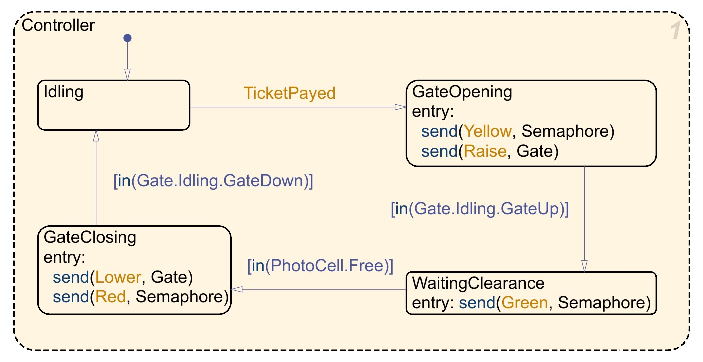
\includegraphics[width=0.8\textwidth]{./img/MATLAB/control_block.pdf}
    \caption{Control Block}
    \label{fig:control_block}
\end{figure}


\paragraph{Gate}

As already mentioned, the \textit{Gate} block is responsible for controlling the gate's position and ensuring that it opens and closes correctly.
It's designed based on two hierarchical states: \textit{Idling} and \textit{Moving}, which then are further divided into \textit{GateUp} and \textit{GateDown} states, and \textit{Raising} and \textit{Lowering} states, respectively.
At first, the \textit{Gate} block is in the \textit{GateDown} state, where the gate is closed and the vehicle is not allowed to pass through.
Once the \textit{Raise} event is received from the \textit{Controller} block, the \textit{Gate} block moves to the \textit{Raising} state, where it starts to open the gate.
Once the gate is fully opened, the \textit{Gate} block moves to the \textit{GateUp} state waiting for the \textit{Lower} event from the \textit{Controller} block that will then perform the same steps in reverse order, moving to the \textit{Lowering} state and then to the \textit{GateDown} state once the gate is fully closed.

Figure \ref{fig:gate_block} shows the \textit{Gate} block of the parking gate FSM.

\begin{figure}[H]
    \centering
    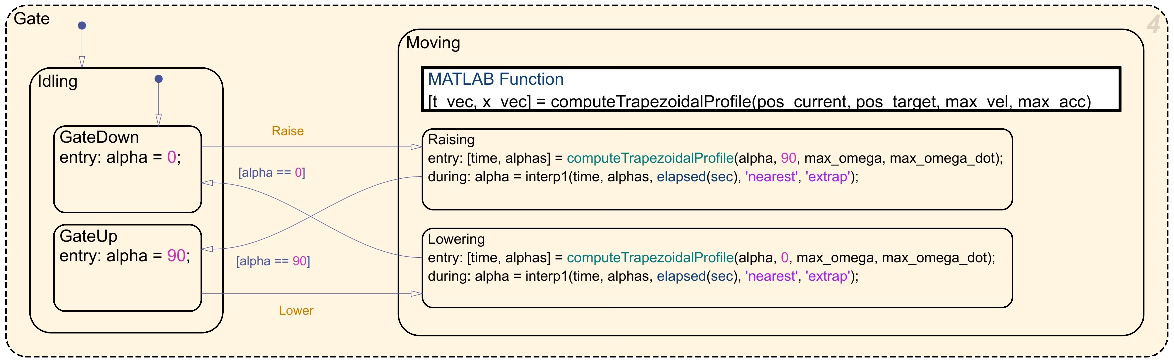
\includegraphics[width=1.0\textwidth]{./img/MATLAB/gate_block.pdf}
    \caption{Gate Block}
    \label{fig:gate_block}
\end{figure}

Notice that, in order to respect the constraints $w_{max} = |4| [^\circ / s]$ and $\dot{w}_{max} = |1| [^\circ / s^2]$, the position of the gate is updated based on the trapezoidal motion profile, generated when entering the \textit{Raising} or \textit{Lowering} states.
The trapezoidal motion profile is defined by the following equations:

\begin{equation}
    w(t) = \begin{cases}
        \frac{w_{max}}{t_1} t                 & 0 \leq t < t_1   \\
        w_{max}                               & t_1 \leq t < t_2 \\
        w_{max} - \frac{w_{max}}{t_3} (t - T) & t_2 \leq t < T
    \end{cases}
\end{equation}

Where $t_1$ is the time when the gate reaches the maximum speed and $t_2$ is the time when the gate starts to decelerate.
The trapezoidal motion profile is designed to ensure that the gate opens and closes smoothly, without any sudden jerks or stops.
Listing \ref{lst:trapezoidal_motion_profile} shows the implementation of the trapezoidal motion profile as MATLAB function.

\begin{lstlisting}[
    style=Matlab-editor,
    caption={Trapezoidal Motion Profile},
    label={lst:trapezoidal_motion_profile}
]
function [t_vec, x_vec] = computeTrapezoidalProfile(pos_current, pos_target, max_vel, max_acc)
% COMPUTE_TRAPEZOIDAL_PROFILE Generates time and angle points for a trapezoidal profile
% At first checks if a trapezoidal profile is feasible or is necessary to
% fallback to a triangular one.

delta_pos = pos_target - pos_current;
time_acc_phase = max_vel / max_acc;
delta_pos_acc_phase = 0.5 * max_acc * time_acc_phase^2;

if 2 * delta_pos_acc_phase < abs(delta_pos)
    % Trapezoidal profile
    t1 = time_acc_phase;
    t2 = (abs(delta_pos) - 2 * delta_pos_acc_phase) / max_vel;
    t3 = time_acc_phase;
else
    % Triangular profile
    max_vel = sqrt(abs(delta_pos) * max_acc);
    t1 = max_vel / max_acc;
    t2 = 0;
    t3 = max_vel / max_acc;
end


% Trapezoidal profile template (HP: s0 = 0, v0 = 0)
acc = max_acc * sign(delta_pos);
vel = max_vel * sign(delta_pos);
profile_template = @(t) ...
    (t <= t1) .*                             (1/2 * acc * t.^2) + ...
    (t > t1 & t <= (t1 + t2)) .*             (1/2 * acc * t1^2 + vel * (t - t1)) + ...
    (t > (t1 + t2) & t <= (t1 + t2 + t3)) .* (1/2 * acc * t1^2 + vel * t2 + vel * (t - (t2 + t1)) - 1/2 * acc * (t - (t1 + t2)).^2) + ...
    (t > (t1 + t2 + t3)) .*                  (1/2 * acc * t1^2 + vel * t2 + vel * t3 - 1/2 * acc * t3.^2);

% Profile generation
t_vec = linspace(0, t1 + t2 + t3, 100);
x_vec = profile_template(t_vec) + pos_current;

end
\end{lstlisting}


\paragraph{PhotoCell}

Despite being used only during the \textit{WaitingClearance} state of the \textit{Controller} block, the \textit{PhotoCell} block is responsible for detecting the vehicle's presence in front of the gate.
This, in fact, is the only way to understand if the vehicle has passed through the gate and the gate can be closed again safely.
In order to continuously sample the vehicle's position, the \textit{PhotoCell} block is designed to not be event-driven, but to move continuously between the two states \textit{Free} and \textit{Occupied} based on the vehicle's position.
By doing so, an external agent can continuously monitor the vehicle's position by checking the state of the \textit{PhotoCell} block.
In order to determines the presence or not of the vehicle, the \textit{PhotoCell} block uses the knowledge of the vehicle's length and position, the latter of which is shared by the \textit{Vehicle FSM}.

Figure \ref{fig:photocell_block} shows the \textit{PhotoCell} block of the parking gate FSM.

\begin{figure}[H]
    \centering
    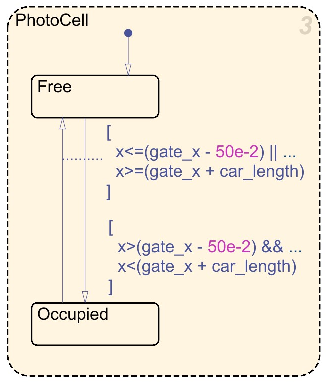
\includegraphics[width=0.4\textwidth]{./img/MATLAB/photocell_block.pdf}
    \caption{PhotoCell Block}
    \label{fig:photocell_block}
\end{figure}


\paragraph{Semaphore}

Last but not least, the \textit{Semaphore} block is responsible for switching the semaphore state between red, yellow and green based on the events received from the \textit{Controller} block.
It has one single state \textit{On} composed of  three sub-states representative of the color of the semaphore.
Based on the event received, the correct sub-state is chosen and the semaphore state is then shared with the \textit{Vehicle FSM} to inform it about the state of the gate (open, closed, etc.).
This is done in order to inform the vehicle about the state of the gate and allow it to proceed or stop based on the semaphore state, which is the only information that the vehicle has about the parking gate system (i.e. the vehicle doesn't know if the gate is open or closed, but only if the semaphore is red or green).

Figure \ref{fig:semaphore_block} shows the \textit{Semaphore} block of the parking gate FSM.

\begin{figure}[H]
    \centering
    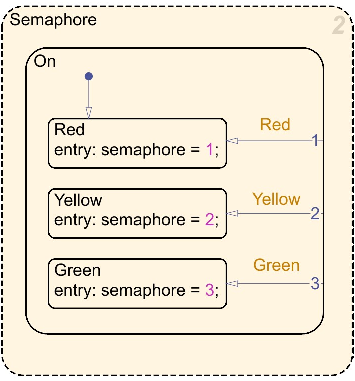
\includegraphics[width=0.4\textwidth]{./img/MATLAB/semaphore_block.pdf}
    \caption{Semaphore Block}
    \label{fig:semaphore_block}
\end{figure}



\subsection{Simulation Results}
\label{subsec:simulation_results}

The simulation has been run for $100s$ and the vehicle has been reset to a new random position right after the closure of the gate.
The following figures show the results of the simulation.

\begin{figure}[H]
    \centering
    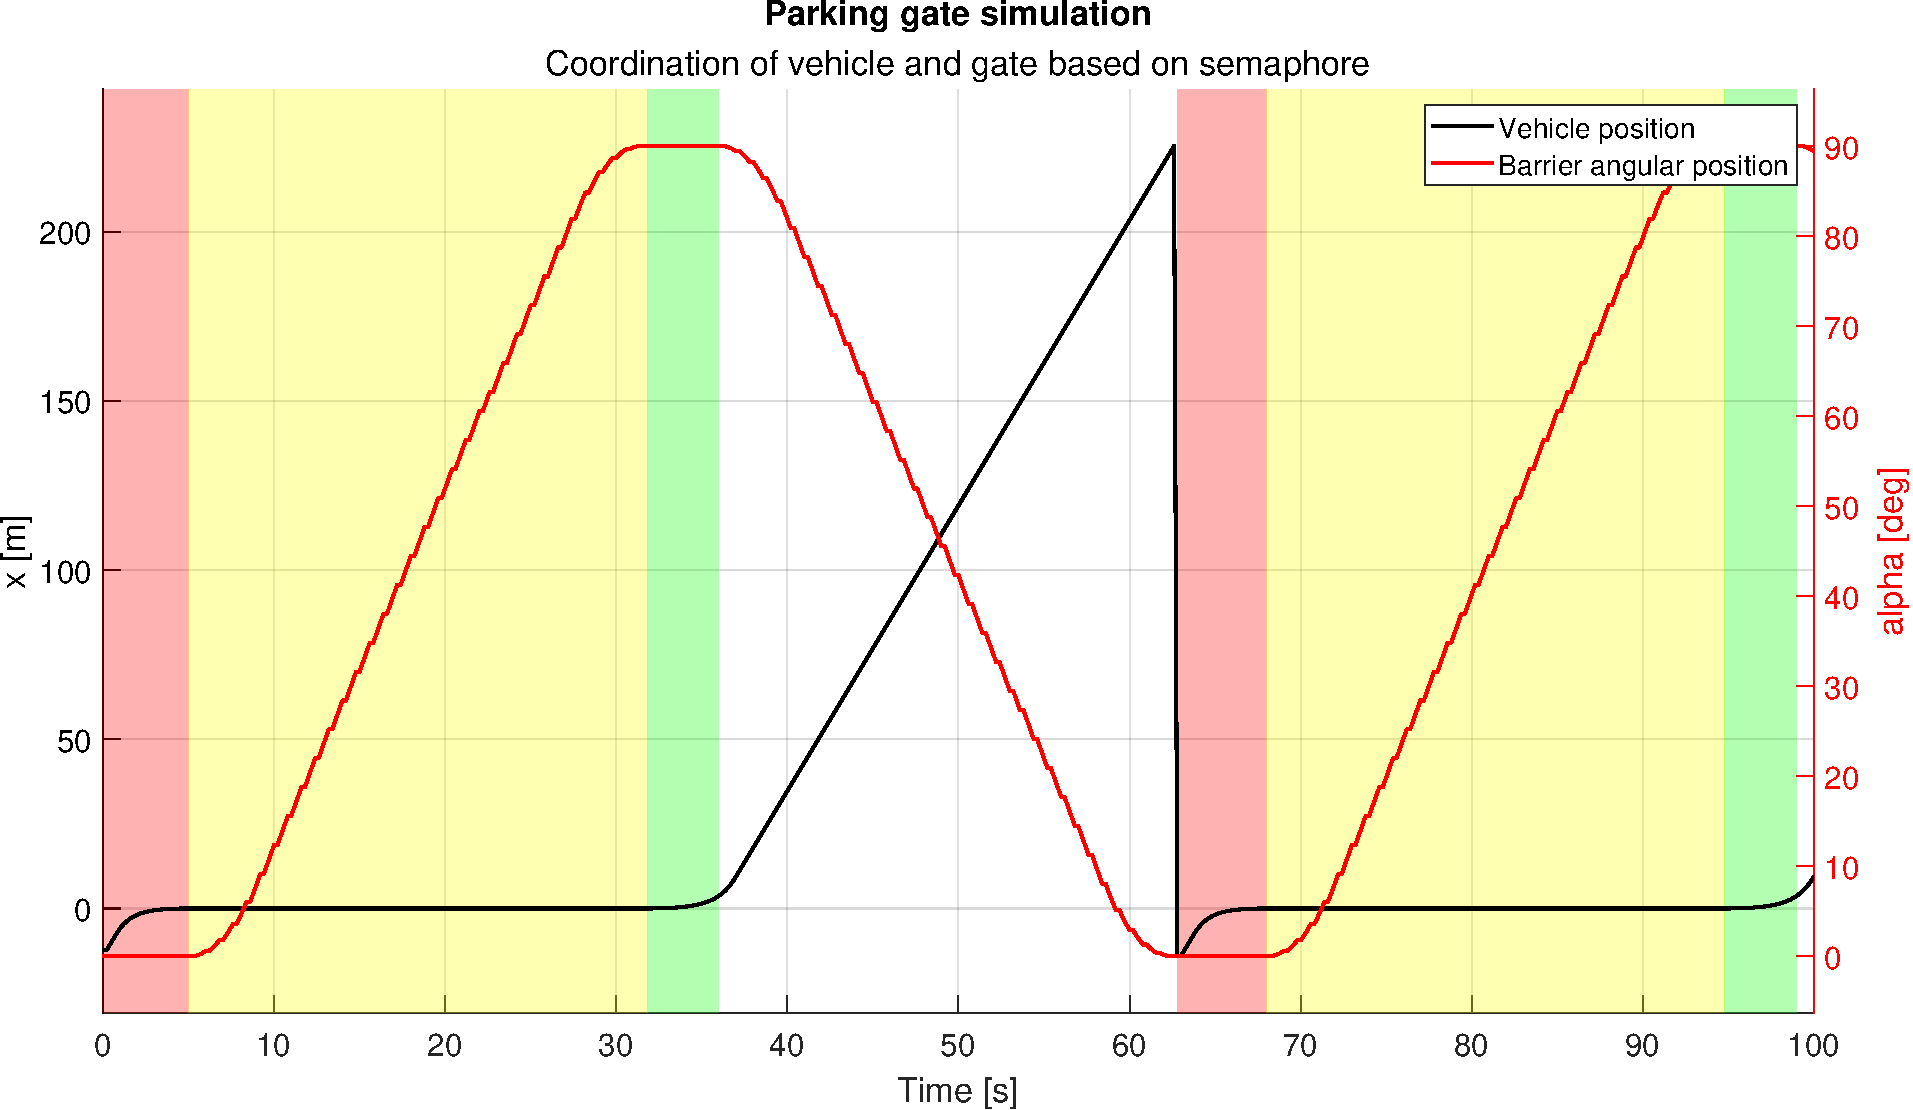
\includegraphics[width=1.0\textwidth]{./img/MATLAB/results.pdf}
    \caption{Simulation Results}
    \label{fig:simulation_results}
\end{figure}

Figure \ref{fig:simulation_results} shows the vehicle position (in black) and the gate angular position (in red) over time.
The plot has also been divided into different regions based on the state of the \textit{Semaphore} block (red, yellow and green).
Notice that for clarity, the semaphore state has been added to the plot only when actually visible by the vehicle (i.e. when the vehicle is in front of the gate and not yet passed through it).

Instead, a more detailed view of the underlying coordination between the two FSMs is shown in Figure \ref{fig:simulation_results_detailed}, where a visualization of the state transitions and events is shown.
The plot report on the vertical axis the time of the simulation and on each vertical dashed line the state of each superstate of the FSMs is shown.
One can appreciate how the two FSMs are coordinated and how the events are sent and received between them, along with the transitions between the states.

\begin{figure}[H]
    \centering
    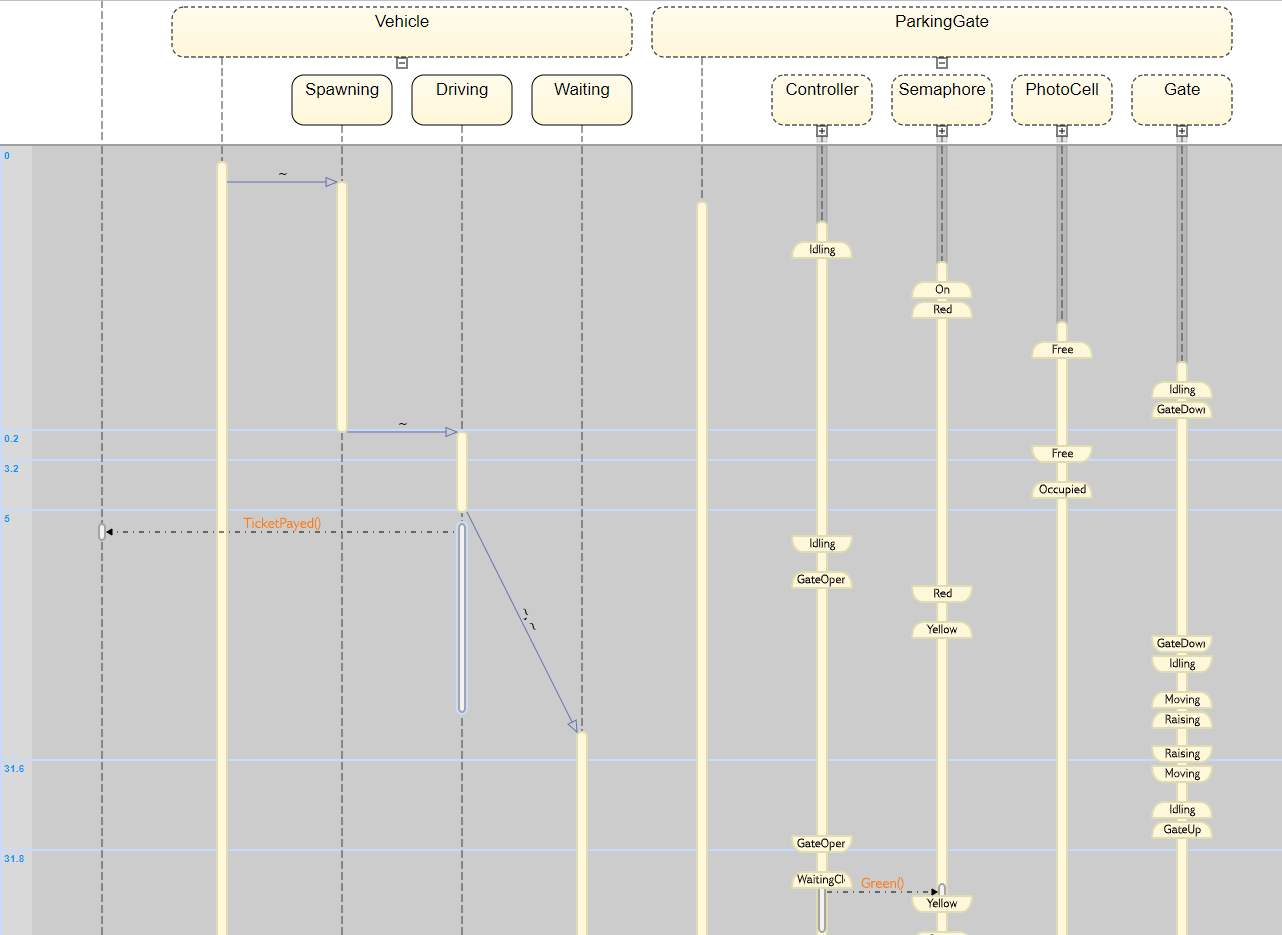
\includegraphics[width=1.0\textwidth]{./img/events_part_1.png}
    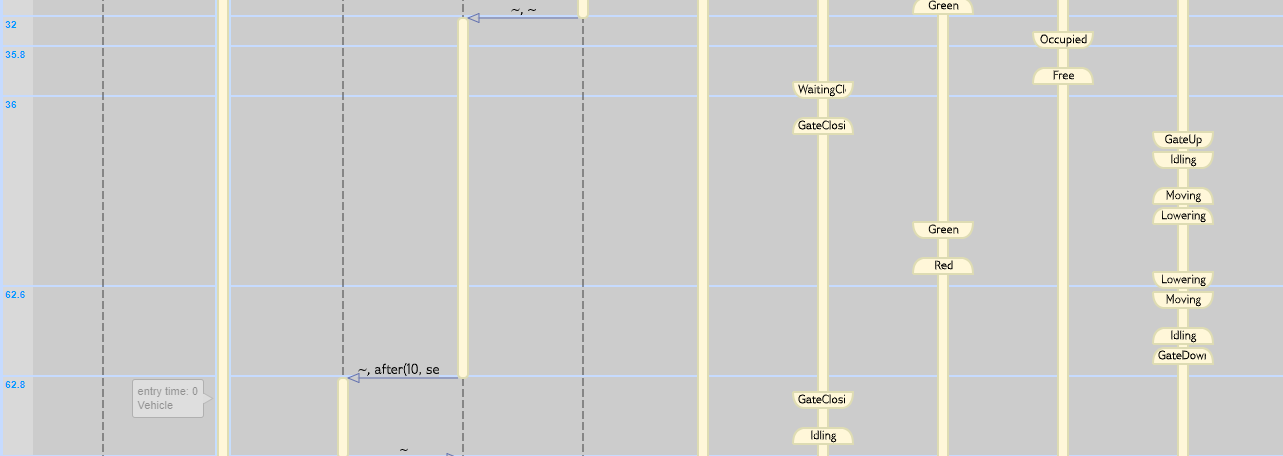
\includegraphics[width=1.0\textwidth]{./img/events_part_2.png}
    \caption{Simulation Results - Detailed View}
    \label{fig:simulation_results_detailed}
\end{figure}










